%====================================================
%================NGƯỜI TẠO: TRẦN THỊNH===============
%==============MẪU DỰ ÁN NHÓM TIKZPRO2020============
%====================================================
\documentclass[11pt,a4paper,onecolumn,titlepage,oneside,openany]{book}
\def\tren{2}\def\duoi{2}\def\trai{2}\def\phai{1.5}
\usepackage[top=\tren cm, bottom=\duoi cm, left=\trai cm, right=\phai cm, headsep=18pt, footskip=26pt] {geometry}
%-------------------------------------
% FONTS CHỮ VÀ CÁC GÓI LỆNH SỬ DỤNG
%-------------------------------------
\usepackage{lmodern}% font mđ Computer Modern
\usepackage[utf8]{vietnam}
\usepackage{fontawesome} % Gói kí hiệu đặc biệt
%=====================================
\usepackage{amsmath,amssymb,mathrsfs,maybemath,xlop,polynom,slashbox}
\usepackage{yhmath} 
\usepackage{enumerate}
\usepackage{tkz-euclide}
\usepackage{tikz-3dplot}
\usepackage{tkz-tab,tkz-linknodes}
%-------------------------------------
\usetikzlibrary{math,through,calc,intersections,angles,quotes,shapes,shapes.geometric,arrows,patterns,snakes,matrix,chains,arrows.meta,decorations.shapes,decorations.fractals,decorations.markings,shadows}
\usetikzlibrary{positioning,decorations.text,decorations.pathmorphing}% Để uốn cong văn bản 
\usetikzlibrary{shadings,fadings} %ĐỔ BÓNG
%\usetkzobj{all}
\usepackage{pgfplots}
\usepackage{pgfornament}
\usepgfplotslibrary{fillbetween}
\pgfplotsset{compat=1.9}
\usepackage[hidelinks,unicode]{hyperref}
\usepackage{currfile}
%--------------Gói trắc nghiệm EX-TEST
%\usepackage[book]{ex_test}
%\usepackage[solcolor]{ex_test} %tô màu đáp án và in lời giải
%\usepackage[dethi]{ex_test} 
\usepackage[loigiai]{ex_test}
%\usepackage[color]{ex_test} %tô màu đáp án và ko in lời giải
%-------Định nghĩa lại hiển thị Lời giải
\def\loigiaiEX{\color{blue!90!black}\fontfamily{pag}\selectfont
	\bfseries\strut
	\faFolderOpen\ 
	Lời giải.}
\fixshowans{vd} 
\newtheorem{vd}{\color{red!70!black}\fontfamily{qag}\selectfont CÂU}
\renewtheorem{ex}{\color{blue}\fontfamily{qag}\selectfont Câu}[vd]
\newenvironment{bt}{\begin{ex}}{\end{ex}}
%---------- Khai báo viết tắt, in đáp án
\newcommand{\hoac}[1]{ %hệ hoặc
	\left[\begin{aligned}#1\end{aligned}\right.}
\newcommand{\heva}[1]{ %hệ và
	\left\{\begin{aligned}#1\end{aligned}\right.}
\usepackage{esvect}
\def\vec{\vv} %vecto
\def\overrightarrow{\vv}
%Lệnh song song
\DeclareSymbolFont{symbolsC}{U}{txsyc}{m}{n}
\DeclareMathSymbol{\varparallel}{\mathrel}{symbolsC}{9}
\DeclareMathSymbol{\parallel}{\mathrel}{symbolsC}{9}
%Kiểu đánh \item
\renewcommand{\labelenumi}{\alph{enumi})}
%Kí hiệu để liệt kê
\def\sao{\color{black} %\faCheckSquareO
	\small\faCheckCircleO}
%====================================
%-----------------------------------Khoanh tròn đáp án khi sd tùy chọn Dethi
\renewcommand{\TrueEX}{\stepcounter{dapan}
	{\circEX{\textbf{\color{blue!30!black}\Alph{dapan}}}} \ignorespaces}
\renewcommand{\FalseEX}{\stepcounter{dapan}
	{\circled{\textbf{\color{blue!30!black}\Alph{dapan}}}} \ignorespaces}
%-------------------------------------
%--------------4.2
\usepackage[most]{tcolorbox}
\colorlet{tcbcol@back}{tcbcolback}
\colorlet{tcbcol@frame}{tcbcolframe}
%---------------
%độ sâu--------------
\setcounter{secnumdepth}{4}
\setcounter{tocdepth}{2}
\usepackage[explicit]{titlesec} % để gọi #1
\usepackage{titledot} % gói lệnh chứa cả titlesec và titletoc
%============================
% Canh chỉnh mục lục chính
%============================
\setcounter{secnumdepth}{4} %Độ sâu đánh số
\setcounter{tocdepth}{2} %Độ sâu mục lục
%===================Làm mục lục
\usepackage{ifoddpage}
\titlecontents{section}
[2.5em]{\sffamily}
{\bfseries\color{blue}\contentslabel{2em}\color{blue}}{}
{\bfseries\color{blue}\dotfill\contentspage\hspace*{1.3ex}}

\titlecontents{subsection}
[4.5em]{\sffamily}
{\color{violet}\contentslabel{2em}\color{violet}}{}
{\color{violet}\dotfill\contentspage\hspace*{1.3ex}}

\makeatletter
\renewcommand*\l@part[2]{%
	\ifnum \c@tocdepth >\m@ne
	\addpenalty{-\@highpenalty}%
	\vskip 1.0em \@plus\p@
	\setlength\@tempdima{1.5em}%
	\begingroup
	\parindent \z@ \rightskip \@pnumwidth
	\parfillskip -\@pnumwidth
	\leavevmode
	\advance\leftskip\@tempdima
	\hskip -\leftskip
	\colorbox{violet}{\strut%
		\makebox[\dimexpr\textwidth-1\fboxsep-6pt\relax][l]{%
			%\fontsize{12pt}{1pt}
			\color{white}\bfseries\fontfamily{qag}\selectfont\hspace*{3cm} #1%
			\nobreak\hfill\nobreak\hb@xt@\@pnumwidth{\hss #2}}}\par\smallskip
	\penalty\@highpenalty
	\endgroup
	\fi}

\renewcommand*\l@chapter[2]{%
	\ifnum \c@tocdepth >\m@ne
	\addpenalty{-\@highpenalty}%
	\vskip 1.0em \@plus\p@
	\setlength\@tempdima{1.5em}%
	\begingroup
	\parindent \z@ \rightskip \@pnumwidth
	\parfillskip -\@pnumwidth
	\leavevmode
	\advance\leftskip\@tempdima
	\hskip -\leftskip
	\colorbox{violet!80}{\strut%
		\makebox[\dimexpr\textwidth-1\fboxsep-6pt\relax][l]{%
			\sffamily%\fontsize{12pt}{1pt}
			\color{white}\bfseries\selectfont Phần #1%
			\nobreak\hfill\nobreak\hb@xt@\@pnumwidth{\hss #2}}}\par\smallskip
	\penalty\@highpenalty
	\endgroup
	\fi}
%---------------------------------------------------------------
% ĐỊNH NGHĨA SECTION. SUBSECTION, SUBSUBSECTION ... THEO Ý RIÊNG
%---------------------------------------------------------------
%=====================================
%\setcounter{secnumdepth}{4} %độ sâu
%\renewcommand\thesection{\@Alph\c@section}
%\renewcommand\thesubsection{\@Roman\c@subsection}
\renewcommand\thesection{\@arabic\c@section}
\renewcommand\thesubsection{\@Alph\c@subsection}
\renewcommand\thesubsubsection{\@arabic\c@subsubsection}
%\renewcommand\thesubsubsection{\@arabic\c@subsubsection}
%=====================================
\definecolor{tsblue}{RGB}{23,74,117}
%--------------------------------Tròn
\newcommand{\tron}[1]{% Định nghĩa hình tròn
	\begin{tikzpicture}[baseline=(A.base)]%
		\node[circle,draw=tsblue,line width=0.5pt,fill=white,inner sep=2pt,outer sep=1pt] (A) {\color{white} #1};
		\node[circle,draw=none,fill=tsblue,inner sep=1pt,outer sep=1pt] (A) {\color{white} #1};
	\end{tikzpicture}%
}
%--------Section------------------------------
\titleformat{\section}
{\fontfamily{put}\fontsize{20pt}{1pt}\selectfont\color{red!80!black}\centering\bfseries}
{D{\fontsize{13pt}{1pt}\selectfont ẠNG }{\fontsize{25pt}{1pt}\selectfont\thesection.}}
{-0.2em}
{
	\setcounter{ex}{0}
	\fontsize{18pt}{1pt}\selectfont\color{red!80!black}\MakeUppercase{#1}
}
[\vspace{0pt}]
%--------------------------------------------
\titleformat{\subsection}
{\fontsize{13pt}{1pt}\fontfamily{qag}\selectfont\bfseries}
{\tron{\thesubsection}}
{0.5em}
{\color{tsblue}\MakeUppercase{#1}
}
%-------------------------------------
\titlespacing{\subsubsection}{0pt}{0cm}{0cm}[0cm]
\titleformat{\subsubsection}
{\color{black}
	\fontsize{12.5pt}{0pt}\sffamily\bfseries}
{\thesubsubsection.}
{0.5em}
{\textcolor{violet!50!black} {#1}}{}
%----------------
%--------------------------------------------
\titlespacing{\chapter}{0cm}{-0.25cm}{0cm}[0cm]
\titleformat{\chapter}[display]
{\normalfont\huge\bfseries}
{}
{0pt}
{
	\begin{tikzpicture}[overlay,remember picture]
		\foreach \ii in {0,1,...,22}{\draw[cyan,line width=2pt,opacity=0.3] 
			([xshift=0.3*\ii cm]current page.north west)--++(-135:10cm)
			;}
	\end{tikzpicture}
	\begin{tikzpicture}[remember picture, overlay,baseline=0cm]
		%-----NODE vị trí (chính)
		\node[inner sep=0pt, %draw=black,
		anchor=west,
		align=right, 
		text width=\textwidth,
		yscale=1.2
		] (chaptername) at (0,0) {
			%		\parbox{15.75cm}{
			\fontsize{23pt}{20pt}\fontfamily{qag}\selectfont\bfseries\color{white}\raggedleft
			\MakeUppercase{#1}
			%		}
		};
		%----Nền
		\fill[draw=tsblue,rounded corners=5pt, fill=red, line width=1pt] ([xshift=-0.1cm,yshift=-0.125cm]chaptername.south east) rectangle ([xshift=5cm,yshift=0.57cm]chaptername.north west);
		%----------
		\fill[draw=tsblue,rounded corners=5pt, fill=red, line width=1pt] ([xshift=4cm,yshift=-0.525cm]chaptername.south west) rectangle ([xshift=0cm,yshift=0cm]chaptername.north west);
		%----------
		\fill[draw=red,rounded corners=5pt, fill=yellow!30, line width=1pt, double,] ([xshift=-0.3cm,yshift=-0.325cm]chaptername.south east) rectangle ([xshift=-0.3cm,yshift=0.325cm]chaptername.north west);
		%-----------
		\node[inner sep=-15pt,
		anchor=west,
		align=right, 
		text width=\textwidth,
		yscale=1.2
		] (chaptername) at (0,0) {
			%		\parbox{15.75cm}{
			\fontsize{23pt}{20pt}\fontfamily{qag}\selectfont\bfseries\color{blue}\raggedleft
			\MakeUppercase{#1}
			%		}	
		};
		%-----tên chương
		\node[inner sep=0pt,left,yscale=1.5,xscale=1.2,right] (tenchuong) at ([xshift=0cm,yshift=1.6cm]chaptername.north west) {\color{violet}\fontsize{15pt}{1pt}\fontfamily{qag}\selectfont\bfseries\MakeUppercase{\chaptername}};
		\node[inner sep=0pt,right,scale=1.85] (chapnum) at ([xshift=0.75cm,yshift=0cm]chaptername.west) {\pgfornament[height=1cm,color=violet]{4}};	
	\end{tikzpicture}
}
[
\vspace{2cm}
\thispagestyle{empty}
]
%============================Mục lục - Chapter*
\makeatletter
\titleformat{name=\chapter,numberless}[display]
{\normalfont\huge\bfseries}
{}
{0.5em}
{%
	\begin{tikzpicture}[remember picture, overlay]%
		\pgftext[right,x=15cm,y=0.2cm]{\color{blue}\fontsize{25pt}{1pt}\fontfamily{qag}\selectfont\bfseries\MakeUppercase{#1}};%
		\draw[fill=blue,draw=blue, rounded corners=15pt] (12.5,-.75) rectangle (20,1.3);%
		\clip (12.5,-.75) rectangle (20,1.3);
		\pgftext[right,x=15cm,y=0.2cm]{\color{white}\fontsize{25pt}{1pt}\fontfamily{qag}\selectfont\bfseries\MakeUppercase{#1}};%
	\end{tikzpicture}
}
[
\vspace{0.5cm}
\thispagestyle{empty}
]
\makeatother
%=============================
\definecolor{tsforestgreen}{RGB}{21,122,81}
\newtcolorbox{note}[1][]{
	enhanced, breakable,
	before skip=3mm,
	after skip=3mm,
	boxrule=1pt,
	left=12mm,right=5mm,top=5mm,bottom=5mm,
	colback=yellow!15,
	colframe=tsforestgreen,
	sharp corners,rounded corners=southeast,arc is angular,arc=3mm,
	underlay={%
		%--phải dưới (nhỏ)
		\path[fill=tsforestgreen!80!black] ([yshift=3mm]interior.south east)--++(-0.4,-0.1)--++(0.1,-0.2);
		\path[draw=tcbcol@frame,shorten <=-0.05mm,shorten >=-0.05mm] ([yshift=3mm]interior.south east)--++(-0.4,-0.1)--++(0.1,-0.2);
		%--trái
		\path[fill=green!20,draw=none] (interior.south west) rectangle node[red!90!black]{
			\fontfamily{qag}\bfseries\fontsize{15}{1}\selectfont !
			%\faExclamationTriangle
		} ([xshift=4mm]interior.north west);
		\draw[draw=tsforestgreen] ([xshift=4mm]interior.south west)-- ([xshift=4mm]interior.north west);
	},
	drop fuzzy shadow, 
	#1}
%----------------------------------
% Hộp định nghĩa
\newenvironment{boxdn}
{\begin{tcolorbox}
		[enhanced jigsaw,breakable,pad at break*=1mm,
		%colback=yellow!5,
		%standard jigsaw, 
		opacityback=0, %ko nền
		boxrule=0pt,frame hidden, left=0.7cm, right=0pt, bottom=2pt, top=0pt,
		borderline west={1mm}{0.5cm}{orange},
		overlay={
			\fill[fill=yellow!20,draw=none] ([xshift=0.6cm]interior.north west) rectangle (interior.south east)
			;
		}
		\setcounter{muccon}{0}
		]}%0mm lề trái
	{\end{tcolorbox}}
%===============================================
\theoremstyle{nonumberbreak} % ko đánh số
\theoremheaderfont{\sffamily\bfseries} %tên
\theorembodyfont{\normalfont} %thân
\theoremsymbol{\ensuremath{_\blacksquare}} %Dấu kết thúc là ô vuông đen.
\theoremseparator {:} % Dấu ngăn cách
\newtheorem{myphantich}{\color{violet}%\faServer\ 
	\faFileText\ PHÂN TÍCH}
%===============================================
\newenvironment{phantich}{\begin{boxdn}\begin{myphantich}}{\end{myphantich}\end{boxdn}}
%==================================
%--------------------------------------
% HEADER AND FOOTER STYLING
%--------------------------------------
\usepackage{fancyhdr,lastpage}
\pagestyle{fancy}
\fancyhf{} 
%======================Đánh số trang, head, foot
\lhead{\it\sf\fontsize{10pt}{1pt}\selectfont\faMortarBoard\, \nouppercase{\leftmark}}
\rhead{\sf\fontsize{10pt}{1pt}\selectfont\faClockO\, Trang \thepage/\pageref{LastPage}}
\lfoot{
	\sf\fontsize{10pt}{1pt}\selectfont\faFileText\, Dự án TeX-50Dang-THPTQG
}
\cfoot{}
\rfoot{\it\sf\nouppercase{\fontsize{10pt}{1pt}\selectfont\faPhoneSquare\ Nhóm TikzPro - Vẽ hình và \LaTeX}}
\renewcommand{\footrulewidth}{0.6pt}
\renewcommand{\headrulewidth}{0.6pt}
%================================================
%----------------------------------------------------
%\usepackage{casio580x}
\usepackage{setspace}
\usepackage{scrextend}
\changefontsizes[17pt]{12pt}%thay đổi font và khoảng cách
\setlength{\parindent}{0pt} %không thụt đầu dòng
%====================================================
\usepackage[final]{pdfpages} % input file bìa pdf
%====================================================
%============================ Khung
\newenvironment{khung}
{\begin{tcolorbox}[
		enhanced,breakable,
		colback=yellow!10,
		colframe=blue,
		boxrule=0.5pt,
		%		drop fuzzy shadow=gray,
		left=5pt,right=5pt,top=5pt,bottom=5pt,
		arc=0mm
		]}
	{\end{tcolorbox}}
%-----------------------------Mục con = subsub
\newcounter{muccon}
\newcommand{\muccon}[1]{%
	\stepcounter{muccon}
	{%\setcounter{bt}{0}\setcounter{vd}{0}\setcounter{ex}{0}
		%\fontsize{13pt}{15pt}\selectfont
		%		\color{violet!70!black}\sffamily
		\bfseries\sffamily\bfseries\hspace*{0mm}\themuccon.\  
		#1}
}
%----------------------------------------------------
%\usepackage{casio580x}
\usepackage{setspace}
\usepackage{scrextend}
%\changefontsizes[20pt]{12pt}%thay đổi font và khoảng cách
\setlength{\parindent}{0pt} %không thụt đầu dòng
%====================================================
\usepackage[final]{pdfpages} % input file bìa pdf
%====================================================
%\hideansEX{vd}% ẩn lời giải môi trường \begin{vd}
%\hideansEX{bt}% ẩn lời giải môi trường \begin{bt}
%\hideansEX{ex}% ẩn lời giải môi trường \begin{ex}
%\dotlineans{10}{vd}% luôn ẩn lời giải và hiện 10 dòng kẻ
%\dotlinefull{ex}% hiện số dòng kẻ bằng số dòng của lời giải
%====================================================
%====================================================
%=================BẮT ĐẦU TÀI LIỆU===================
\begin{document}
	%\pagenumbering{arabic}
	%\pagenumbering{roman}%đánh số trang kiểu la mã
	\renewcommand{\chaptername}{Chuyên đề} %thay đổi chương
	%=====================mục lục
	\pagenumbering{gobble}%tắt đánh số trang
	
\includepdf[]{biasach/biasach-so5-ban1.pdf}%chèn bìa pdf
	%\newpage\null\thispagestyle{empty}\newpage%tạo trang trống
	\pagenumbering{roman}%đánh số trang dạng i,ii,...
	%~~~~~~~~~~~~~~~~~~~~~
	\tableofcontents %lệnh in mục lục chính
	\clearpage%đặt lại đánh số trang
	\pagenumbering{arabic}%đánh số trang dạng 1,2,...
%====================================================
\chapter{50 dạng toán THPT Quốc Gia}
	%Dạng 1
\section{Phép đếm}
\subsection{Kiến thức cần nhớ}
\begin{khung}
	\subsubsection{Quy tắc cộng} Một công việc được hoàn thành bời một trong hai hành động. Nếu hành động này có $m$ cách thực hiện, hành động kia có $n$ cách thực hiện không trùng với bất kì cách nào của hành động thứ nhất thì công việc đó có $m + n$ cách thực hiện.
	\begin{itemize}
		\item Nếu $A$ và $B$ là các tập hợp hữu hạn không giao nhau thì: $n(A\cup B)=n(A)+n(B)$.
	\end{itemize}
	\subsubsection{Quy tắc nhân} Một công việc được hoàn thành bởi hai hành động liên tiếp. Nếu có $m$ cách thực hiện hành động thứ nhất và ứng với mỗi cách đó có $n$ cách thực hiện hành động thứ hai thì có $m\cdot n$ cách hoàn thành công việc.
	\begin{itemize}
		\item Dạng toán tìm số các số tạo thành: Gọi số cần tìm có dạng: $\overline{abc\ldots}$, tuỳ theo yêu cầu bài toán:\\
		Nếu số lẻ thì số tận cùng là số lẻ.\\
		Nếu số chẵn thì số tận cùng là số chẵn.
	\end{itemize}
\end{khung}
\subsection{Bài tập mẫu}
\Opensolutionfile{ans}[ans/ANS-DANG-1]
\begin{vd}%[Nguyễn Tấn Linh]%[2H2B1-1]
	[Đề minh họa BDG 2019-1020] 
	Từ một nhóm học sinh $6$ nam và $8$ nữ. Có bao nhiêu cách chọn ra một học sinh?
	\choice
	{\True $14$}	
	{$48$}
	{$6$}
	{$8$}
	\loigiai{
	\begin{phantich}
		\muccon{Dạng toán:}
			Đây là dạng toán quy tắc đếm, cụ thể là quy tắc cộng.\\
		\muccon{Hướng giải:}
			\begin{enumerate}[\bf B1.]
				\item Số cách chọn $1$ học sinh nữ từ $8$ học sinh nữ có $8$ cách.
				\item Số cách chọn $1$ học sinh nam từ $6$ học sinh nam có $6$ cách. 
				\item Số cách chọn ra một học sinh là $8+6=14$.
			\end{enumerate}
			Từ đó, ta có thể giải bài toán cụ thể như sau:
	\end{phantich}
	\textit{Cách 1.} Số cách chọn $1$ học sinh nữ từ $8$ học sinh nữ có $8$ cách.\\
	Số cách chọn $1$ học sinh nam từ $6$ học sinh nam có $6$ cách Số cách chọn ra một học sinh là $8+6=14$.\\
	\textit{Cách 2.} Tổng số học sinh là $8+6=14$.\\
	Số cách chọn $1$ học sinh nữ từ $14$ học sinh có $14$ cách.
	}
\end{vd}
\subsection{Bài tập tương tự và phát triển}
%%==========Câu 1
\begin{ex}%[Nguyễn Tấn Linh]%[1D2Y1-1]
	Trong một hộp chứa sáu quả cầu trắng được đánh số từ $1$ đến $6$ và ba quả cầu đen được đánh số từ $7$ đến $9$. Có bao nhiêu cách chọn một trong các quả cầu ấy?
	\choice
	{$1$}
	{$3$}
	{$6$}
	{\True $9$}
	\loigiai{
		Mỗi quả cầu được đánh một số khác nhau, nên mỗi lần lấy ra một quả cầu bất kì là một lần.\\
		Số quả cầu là $6+3=9$.\\
		Tương ứng với $9$ cách.}
\end{ex}
%%==========Câu 2
\begin{ex}%[Nguyễn Tấn Linh]%[1D2Y1-1]
	Lớp 12A có 43 học sinh, lớp 12B có 30 học sinh. Chọn ngẫu nhiên 1 học sinh từ lớp 12A và 12B. Hỏi có bao nhiêu cách?
	\choice
	{\True $43$}
	{$30$}
	{$73$}
	{$1290$}
	\loigiai{
		Tổng số học sinh 2 lớp là $43+30=73$.\\
		Số cách chọn là 73.}
\end{ex}
%%==========Câu 3
\begin{ex}%[Nguyễn Tấn Linh]%[1D2Y1-1]
	Từ các chữ số $1, 2, 3, 4$ có thể lập được bao nhiêu số tự nhiên gồm $1$ chữ số?
	\choice
	{$5$}
	{$3$}
	{$1$}
	{\True $4$}
	\loigiai{
		Số tự nhiên cần lập có $1$ chữ số được lấy ra từ $4$ số trên, do đó có $4$ cách.}
\end{ex}
%%==========Câu 4
\begin{ex}%[Nguyễn Tấn Linh]%[1D2Y1-2]
	Bạn muốn mua một cây bút mực và một cây bút chì. Các cây bút mực có $8$ màu khác nhau, các cây bút chì cũng có $8$ màu khác nhau. Như vậy bạn có bao nhiêu cách?
	\choice
	{$16$}
	{$2$}
	{\True $64$}
	{$3$}
	\loigiai{
		Mua một cây bút mực có $8$ cách.\\
		Mua một cây bút chì có $8$ cách.\\
		Công việc mua bút là hành động liên tiếp, theo quy tắc nhân ta có $8.8=64$ cách.}
\end{ex}
%%==========Câu 5
\begin{ex}%[Nguyễn Tấn Linh]%[1D2Y1-1]
	Bạn cần mua một cây bút để viết bài. Bút mực có 8 loại khác nhau, bút chì có 8 loại khác nhau. Như vậy bạn có bao nhiêu cách?
	\choice
	{\True $16$}
	{$2$}
	{$64$}
	{$3$}
	\loigiai{
		Công việc mua bút có $2$ phương án độc lập nhau.\\
		Phương án 1 mua một cây bút mực có $8$ cách.\\
		Phương án 2 mua một cây bút chì có $8$ cách.\\
		Theo quy tắc cộng, ta có: $8+8=16$ cách.}
\end{ex}
%%==========Câu 6
\begin{ex}%[Nguyễn Tấn Linh]%[1D2Y1-2]
	Từ thành phố A có 10 con đường đến thành phố B, từ thành phố B có 7 con đường đến thành phố C. Từ A đến C phải qua B, hỏi có bao nhiêu cách đi từ A đến C?
	\choice
	{$10$}
	{$7$}
	{$17$}
	{\True $70$}
	\loigiai{
		Công việc đi từ A đến C gồm $2$ hành động liên tiếp.\\
		Hành động 1: đi từ A đến B có 10 cách.\\
		Hành động 2: đi từ B đến C có 7 cách.\\
		Theo quy tắc nhân, đi từ A đến C có $10\cdot 7=70$ cách.}
\end{ex}
%%==========Câu 7
\begin{ex}%[Nguyễn Tấn Linh]%[1D2Y1-3]
	Từ thành phố A có 10 con đường đi đến thành phố B, từ thành phố A có 9 con đường đi đến thành phố C, từ thành phố B đến thành phố D có 6 con đường, từ thành phố C đến thành phố D có 11 con đường và không có con đường nào nối B với C. Hỏi có bao nhiêu cách đi từ thành phố A đến thành phố D?
	\choice
	{$156$}
	{\True $159$}
	{$162$}
	{$176$}
	\loigiai{
		\begin{center}
			\begin{tikzpicture}[>=stealth,line join=round,line cap=round,font=\footnotesize,scale=1]
			\coordinate[label=above left:$A$](A) at (0,0);
			\coordinate[label=above:$B$](B) at (3,0); 
			\coordinate[label=below :$C$](C) at (2,-2);
			\coordinate[label=right:$D$](D) at (5,-1);
			\draw[line width=0.7pt,black] (A)--(B)node[above,pos=0.5]{10 con đường}; 
			\draw[line width=0.7pt,black] (B)--(D)node[above right,pos=0.5]{6 con đường};
			\draw[line width=0.7pt,black] (A)--(C)node[right,pos=0.5]{9 con đường};
			\draw[line width=0.7pt,black] (C)--(D)node[below right,pos=0.5]{11 con đường};
			\end{tikzpicture}
		\end{center}
		Phương án 1: đi từ A đến B rồi đến D.\\
		Đây là hành động liên tiếp nên ta áp dụng quy tắc nhân: $10\cdot 6=60$.\\
		Phương án 2: đi từ A đến C rồi đến D.\\
		Tương tự ta áp dụng quy tắc nhân: $9\cdot11=99$.\\
		Hai phương án độc lập nhau nên ta áp dụng quy tắc cộng.\\
		$60+99=159$ cách.}
\end{ex}
%%==========Câu 8
\begin{ex}%[Nguyễn Tấn Linh]%[1D2Y1-2]
	Trong một giải đấu bóng đá có $20$ đội tham gia với thể thức thi đấu vòng tròn. Cứ hai đội thì gặp nhau đúng một lần. Hỏi có tất cả bao nhiêu trận đấu xảy ra?
	\choice
	{$120$}
	{$39$}
	{$380$}
	{\True $190$}
	\loigiai{
		Mỗi đội phải đấu với 19 đội còn lại, nên theo quy tắc nhân ta có $19\cdot 20=380$ trận.\\
		Nhưng đội A gặp đội B thì được tính hai lần. Do đó số trận đấu thực tế là $\dfrac{380}{2}=190$ trận.}
\end{ex}
%%==========Câu 9
\begin{ex}%[Nguyễn Tấn Linh]%[1D2Y1-2]
	Một người vào cửa hàng ăn, người đó chọn thực đơn gồm 1 món ăn trong 5 món, 1 loại quả trong 5 loại, 1 loại nước uống trong 3 loại. Hỏi có bao nhiêu cách lập thực đơn?
	\choice
	{$73$}
	{\True $75$}
	{$85$}
	{$95$}
	\loigiai{
		Lập thực đơn gồm 3 hành động liên tiếp:\\
		Chọn món ăn có 5 cách.\\
		Chọn quả có 5 cách.\\
		Chọn nước uống có 3 cách.\\
		Theo quy tắc nhân: $5\cdot5\cdot3=75$ cách.}
\end{ex}
%%==========Câu 10
\begin{ex}%[Nguyễn Tấn Linh]%[1D2Y1-1]
	Cho hai tập hợp $A=\{a,b,c,d\}$;  $B=\{e,f,g\}$. Kết quả của $n(A\cup B)$ là
	\choice
	{\True $7$}
	{$5$}
	{$8$}
	{$9$}
	\loigiai{
		Ta có $A\cap B=\emptyset$ nên $A$ và $B$ rời nhau.\\
		$n(A\cup B)=n(A)+n(B)=4+3=7$.}
\end{ex}
%%==========Câu 11
\begin{ex}%[Nguyễn Tấn Linh]%[1D2Y1-3]
	Cho hai tập hợp $A=\{a,b,c,d\}; B=\{c,d,e\}$. Kết quả của $n(A\cup B)$ là
	\choice
	{$7$}
	{\True $5$}
	{$8$}
	{$9$}
	\loigiai{
		Ta có $A\cap B=\{c,d\}\Rightarrow n(A\cap B)=2$.\\
		$n(A\cup B)=n(A)+n(B)-n(A\cap B)$.\\
		$n(A\cup B)=4+3-2=5$.}
\end{ex}
%%==========Câu 12
\begin{ex}%[Nguyễn Tấn Linh]%[1D2Y1-3]
	Có bao nhiêu hình vuông trong hình dưới đây?
	\begin{center}
		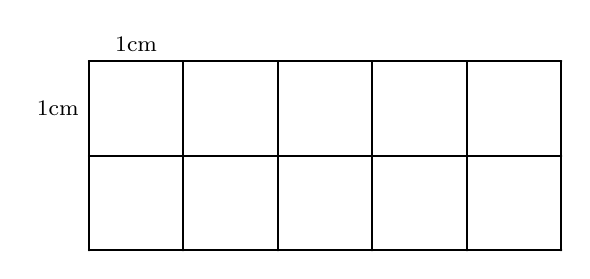
\begin{tikzpicture}[>=stealth,line join=round,line cap=round,font=\footnotesize,scale=0.6]
		\coordinate (A) at (0,0);
		\coordinate (B) at (2,0);
		\coordinate (C) at (4,0);
		\coordinate (D) at (6,0);
		\coordinate (E) at (8,0);
		\coordinate (F) at (10,0);
		\coordinate (A-1) at (0,-2);
		\coordinate (F-1) at (10,-2);
		\coordinate (A-2) at (0,-4);
		\coordinate (B-2) at (2,-4);
		\coordinate (C-2) at (4,-4);
		\coordinate (D-2) at (6,-4);
		\coordinate (E-2) at (8,-4);
		\coordinate (F-2) at (10,-4);
		\draw[line width=0.7pt,black] (A)--(F);
		\draw[line width=0.7pt,black] (A-1)--(F-1);
		\draw[line width=0.7pt,black] (A-2)--(F-2);
		\draw[line width=0.7pt,black] (A)--(A-2);
		\draw[line width=0.7pt,black] (B)--(B-2);
		\draw[line width=0.7pt,black] (C)--(C-2);
		\draw[line width=0.7pt,black] (D)--(D-2);
		\draw[line width=0.7pt,black] (E)--(E-2);
		\draw[line width=0.7pt,black] (F)--(F-2);
		\draw[line width=0.7pt,black] (A)--(B)node[above,pos=0.5]{1cm};
		\draw[line width=0.7pt,black] (A)--(A-1)node[left,pos=0.5]{1cm};
		\end{tikzpicture}
	\end{center}
	\choice
	{\True $14$}
	{$12$}
	{$10$}
	{$5$}
	\loigiai{
		Gọi $A$ là tập hợp hình vuông có cạnh $1$ cm.\\
		$B$ là tập hợp hình vuông có cạnh $2$ cm.\\
		$A$ và $B$ là hai tập hợp rời nhau.\\
		Số hình vuông trong hình là $n(A\cup B)=n(A)+n(B)=10+4=14$.}
\end{ex}
%%==========Câu 13
\begin{ex}%[Nguyễn Tấn Linh]%[1D2Y1-3]
	Từ các chữ số $1,2,3,4,5,6$ có thể lập được bao nhiêu số tự nhiên bé hơn $100$?
	\choice
	{\True $42$}
	{$54$}
	{$62$}
	{$36$}
	\loigiai{
		TH1: Số tự nhiên có một chữ số: 6 số.\\
		TH2: Số tự nhiên có hai chữ số:\\
		Ta đặt là $\overline{ab}$.\\
		Ta có: $6\cdot6=36$ số thoả mãn.\\
		Vậy số số tự nhiên thoả yêu cầu bài toán là $6+36=42$.}
\end{ex}
%%==========Câu 14
\begin{ex}%[Nguyễn Tấn Linh]%[1D2Y1-3]
	Trong mặt phẳng toạ độ $Oxy$, ở góc phần tư thứ nhất ta lấy $2$ điểm phân biệt; cứ thế ở các góc phần tư thứ hai, thứ ba, thứ tư lần lượt lấy $3,4,5$ điểm phân biệt (các điểm không nằm trên các trục toạ độ). Trong 14 điểm đó ta lấy $2$ điểm bất kỳ và nối chúng lại, hỏi có bao nhiêu đoạn thẳng cắt hai trục toạ độ, biết đoạn thẳng nối 2 điểm bất kì không qua $O$. 
	\choice
	{$91$}
	{$42$}
	{$29$}
	{\True $23$}
	\loigiai{
		\begin{center}
			\begin{tikzpicture}[>=stealth,line join=round,line cap=round,font=\footnotesize,scale=1]
			\draw[->] (-4,0)--(4,0)node[below]{$x$};
			\draw[->] (0,-4)--(0,4)node[right]{$y$};
			\fill (0,0)node[below left]{$O$}circle(1pt);
			\coordinate[label=above:$A$](A) at (2,3); 
			\coordinate[label=right:$B$](B) at (3,2);
			\coordinate[label=below left:$C$](C) at (-2,3.5);
			\coordinate[label=below left:$D$](D) at (-3,2.5);
			\coordinate[label=below left:$E$](E) at (-1,1);
			\coordinate[label=below left:$F$](F) at (-3,-1);
			\coordinate[label=below left:$G$](G) at (-2,-1.5);
			\coordinate[label=below left:$H$](H) at (-2.5,-2.5);
			\coordinate[label=below left:$I$](I) at (-3.5,-2);
			\coordinate[label=below left:$J$](J) at (2,-1);
			\coordinate[label=below left:$K$](K) at (3,-1.5);
			\coordinate[label=below left:$M$](M) at (1.5,-2);
			\coordinate[label=below left:$L$](L) at (2.5,-3);
			\coordinate[label=below left:$N$](N) at (1.5,-3.5);
			
			\fill[black](A)circle (1.5pt);
			\fill[black](B)circle (1.5pt);
			\fill[black](C)circle (1.5pt);
			\fill[black](D)circle (1.5pt);
			\fill[black](E)circle (1.5pt);
			\fill[black](F)circle (1.5pt);
			\fill[black](G)circle (1.5pt);
			\fill[black](H)circle (1.5pt);
			\fill[black](I)circle (1.5pt);
			\fill[black](J)circle (1.5pt);
			\fill[black](K)circle (1.5pt);
			\fill[black](L)circle (1.5pt);
			\fill[black](M)circle (1.5pt);
			\fill[black](N)circle (1.5pt);
			
			\draw[line width=0.7pt,black] (B)--(A)--(D)  (G)--(A)--(J);
			
			\end{tikzpicture}
		\end{center}
		Để chọn $2$ điểm trong $14$ điểm đã cho nối lại cắt hai trục toạ độ thì hai điểm đó phải thuộc hai góc phần tư đối đỉnh với nhau.\\
		TH1: Chọn 1 điểm ở góc phần tư thứ I và 1 điểm ở góc phần tư thứ III.\\
		Số đoạn thẳng tạo thành: $2.4=8$.\\
		TH2: Chọn 1 điểm ở góc phần tư thứ II và 1 điểm ở góc phần tư thứ IV.\\
		Số đoạn thẳng tạo thành: $3.5=15$.\\
		Theo quy tắc cộng ta có $8+15=23$ đoạn thẳng.}
\end{ex}
%%==========Câu 15
\begin{ex}%[Nguyễn Tấn Linh]%[1D2Y1-3]
	Cho tập hợp số $A=\left\{0,1,2,3,4,5,6\right\}$. Hỏi có thể lập thành bao nhiêu số có 4 chữ số khác nhau và chia hết cho $3$?
	\choice
	{$114$}
	{\True $144$}
	{$146$}
	{$148$}
	\loigiai{
		Ta có một số chia hết cho $3$ khi và chỉ khi tổng các chữ số của nó chia hết cho $3$.\\
		Trong tập $A$, các tập con có 4 chữ số chia hết cho $3$ là\\
		$\{0,1,2,3\},\{0,1,2,6\}$, $\{0,2,3,4\}$, $\{0,3,4,5\}$, $\{1,2,4,5\}$, $\{1,2,3,6\}$, $\{1,3,5,6\}$.\\
		Xét bộ số $\{0,1,2,3\}$, số số có $4$ chữ số khác nhau được tạo thành từ bộ này là $3\cdot3\cdot 2\cdot 1=18$.\\
		Tương tự các bộ $\{0,1,2,6\}$, $\{0,2,3,4\}$, $\{0,3,4,5\}$ cũng lập được 18 số.\\
		Xét bộ số $\{1,2,4,5\}$, số số có $4$ chữ số khác nhau được tạo thành từ bộ này là $4\cdot3\cdot 2\cdot 1=24$.\\
		Tương tự cách bộ $\{1,2,3,6\}$, $\{1,3,5,6\}$ cũng lập được $24$ số.\\
		Vậy số số thoả yêu cầu bài toán là $18\cdot 4+24\cdot 3=144$.}
\end{ex}
%%==========Câu 16
\begin{ex}%[Nguyễn Tấn Linh]%[1D2Y1-2]
	Từ các chữ số $1,2,3,4$ có thể lập được bao nhiêu số tự nhiên có $3$ chữ số khác nhau?
	\choice
	{\True $24$}
	{$9$}
	{$64$}
	{$4$}
	\loigiai{
		Gọi số tự nhiên có $3$ chữ số cần lập có dạng $\overline{abc}$.\\
		$a$ có $4$ cách chọn (từ $1,2,3,4$).\\
		$b$ có $3$ cách chọn (từ $1,2,3,4$ trừ số $a$ đã chọn).\\
		$c$ có $2$ cách chọn (từ $1,2,3,4$ trừ số $a, b$ đã chọn).\\
		Theo quy tắc nhân, ta có: $4\cdot3\cdot 2=24$ cách.}
\end{ex}
%%==========Câu 17
\begin{ex}%[Nguyễn Tấn Linh]%[1D2B1-2]
	Từ các chữ số $1,2,3,4,5,6,7$ lập được bao nhiêu số tự nhiên gồm 4 chữ số khác nhau và là số chia hết cho 5?
	\choice
	{$180$}
	{\True $120$}
	{$360$}
	{$216$}
	\loigiai{
		Gọi số có $4$ chữ số cần lập có dạng $\overline{abcd}$.\\
		Để số lập được chia hết cho $5$ thì số tận cùng phải chia hết cho $5$, khi đó\\
		$d=5$, có 1 cách chọn.\\
		$a$ có $6$ cách\\
		$b$ có $5$ cách\\
		$c$ có $4$ cách\\
		Theo quy tắc nhân ta có: $1\cdot6\cdot 5\cdot 4=120$ cách.}
\end{ex}
%%==========Câu 18
\begin{ex}%[Nguyễn Tấn Linh]%[1D2B1-2]
	Từ các số $1,2,3,4,5,6,7$ lập được bao nhiêu số tự nhiên lẻ gồm 4 chữ số khác nhau?
	\choice
	{$180$}
	{\True $480$}
	{$360$}
	{$120$}
	\loigiai{
		Gọi số có $4$ chữ số cần lập có dạng $\overline{abcd}$.\\
		Số lập được là số lẻ thì số tận cùng là số lẻ $\Rightarrow d \in\{1,3,5,7\}$, suy ra:\\
		$d$ có $4$ cách\\
		$a$ có $6$ cách\\
		$b$ có $5$ cách\\
		$c$ có $4$ cách\\
		Theo quy tắc nhân ta có: $4\cdot6\cdot5\cdot4=480$ cách.}
\end{ex}
%%==========Câu 19
\begin{ex}%[Nguyễn Tấn Linh]%[1D2B1-3]
	Cho tập hợp $A=\left\{0,1,2,3,4,5,6\right\}$. Từ tập $A$ có thể lập được bao nhiêu số tự nhiên gồm $5$ chữ số chia hết cho $5$?
	\choice
	{\True $660$}
	{$420$}
	{$679$}
	{$523$}
	\loigiai{
		Gọi số có $5$ chữ số cần lập có dạng $\overline{abcde}$.\\
		Trường hợp 1: $e=0$, suy ra\\
		$a$	có $6$ cách chọn\\
		$b$	có $5$ cách chọn\\
		$c$	có $4$ cách chọn\\
		$d$ có $3$ cách chọn\\
		$e$ có $1$ cách chọn.\\
		Theo quy tắc nhân ta có: $6\cdot5\cdot4\cdot3\cdot1=360$ cách.\\
		Trường hợp 2: $e=5$, suy ra\\
		$a$ có $5$ cách chọn\\
		$b$ có $5$ cách chọn\\
		$c$ có $4$ cách chọn\\
		$d$ có $3$ cách chọn\\
		$e$ có $1$ cách chọn.\\
		Theo quy tắc nhân ta có: $5\cdot5\cdot4\cdot3\cdot1=300$ cách.\\
		Theo quy tắc cộng, ta có $360+300=660$ cách.}
\end{ex}
%%==========Câu 20
\begin{ex}%[Nguyễn Tấn Linh]%[1D2G1-3]
	Hỏi có tất cả bao nhiêu số tự nhiên chia hết cho $9$ mà mỗi số gồm $2011$ chữ số và trong đó có ít nhất hai chữ số $9$?
	\choice
	{$10^{2010}-16151\cdot 9^{2008}$}
	{$10^{2010}-16153\cdot 9^{2008}$}
	{$10^{2010}-16148\cdot 9^{2008}$}
	{\True $10^{2010}-16161\cdot 9^{2008}$}
	\loigiai{
		Đặt $A_1=\{0;9\}; A_2=\{1\}; A_3=\{2\}; A_4=\{3\};A_5=\{4\};A_6=\{5\};A_7=\{6\};A_8=\{7\}; A_9=\{8\}$.\\
		Gọi số cần tìm là $n=\overline{a_1a_2\ldots a_{2010}a_{2011}}\quad(a_1\neq 0)$.
		\begin{itemize}
			\item Xét các số tự nhiên chia hết cho 9, gồm 2011 chữ số
			\begin{itemize}
				\item Mỗi vị trí từ $a_2$ đến $a_{2011}$ đều có 10 cách chọn.
				\item $a_1$ phụ thuộc vào tổng $\left(a_2+a_3+\cdots +a_{2011}\right)$ nên có 1 cách chọn.
			\end{itemize}
			Vậy có $10^{2010}$ số.
			\item Xét các số tự nhiên chia hết cho 9, gồm 2011 chữ số nhưng không có mặt chữ số 9.
			\begin{itemize}
				\item $a_1$ có 8 cách chọn.
				\item Từ $a_2$ đến $a_{2010}$, mỗi vị trí đều có 9 cách chọn.
				\item $a_{2011}$ có 1 cách chọn.
			\end{itemize}
			Vậy có $8\cdot9^{2009}$ số.
			\item Xét các số tự nhiên chia hết cho 9, gồm 2011 chữ số trong đó có đúng 1 chữ số 9.
			\begin{itemize}
				\item Trường hợp $a_1=9$ ta có:
				\begin{itemize}
					\item Từ $a_2$ đến $a_{2010}$, mỗi vị trí đều có 9 cách chọn.
					\item $a_{2011}$ có 1 cách chọn.
				\end{itemize}
				Do đó có $9^{2009}$ số.
				\item Trường hợp $a_1\neq 9$ ta có:
				\begin{itemize}
					\item $a_1$ có 8 cách chọn.
					\item Có 2010 cách xếp chữ số 9.
					\item Ở 2008 vị trí còn lại, mỗi vị trí có 9 cách chọn.
					\item Vị trí cuối cùng có 1 cách chọn.
				\end{itemize}
				Do đó có $8.2010\cdot 9^{2008}$ số.
			\end{itemize}
		\end{itemize}
		Vậy số các số tự nhiên thỏa mãn yêu cầu bài toán là
		$$10^{2010}-\left(8\cdot 9^{2009}+9^{2009}+8\cdot2010\cdot9^{2008}\right)=10^{2010}-16161\cdot 9^{2008}\text{ số.}$$
	}
\end{ex}
\Closesolutionfile{ans}
%======================
\subsection{Bảng đáp án}
\inputansbox{10}{ans/ANS-DANG-1}



\end{document}